%!TEX root = main.tex

Para realizar la aplicación de la teoría anteriormente explicada, utilizamos Google Colab y Python, junto con las librerías \texttt{unireedsolomon}, \texttt{biopython}, \texttt{matplotlib}, \texttt{py3Dmol} y \texttt{nglview}.\\
Inicialmente para dar un contexto de las estructuras que estamos utilizando, através de \texttt{py3Dmol} y \texttt{nglview} mostramos el modelo de ADN.Posteriormente, utilizando la librería \texttt{biopython}, para una cadena de ADN, mostramos cuál sería su cadena complementaria y la inversa de esta. Esto nos permite ilustrar cómo estas cadenas están anidadas entre sí. Esta aplicación la hicimos através del siguiente código 

\begin{lstlisting}[language=Python]
from Bio.Seq import Seq 
from Bio.SeqUtils import gc_fraction

# Aqui poner la cadena que quieran
cadena_adn = Seq("AGCTAGCTAGCTAAGCTGTA")

# cadena complementaria
cadena_complementaria = cadena_adn.complement()

# inversa complementaria o cadena opuesta
cadena_inversa_complementaria = cadena_adn.reverse_complement()

print("Cadena ADN: ", cadena_adn)
print("Cadena complementaria: ", cadena_complementaria)
print("Cadena inversa complementaria: ", cadena_inversa_complementaria)
\end{lstlisting}
lo cual se puede ilustrar de la siguiente manera
\begin{figure}[h]
\centering
        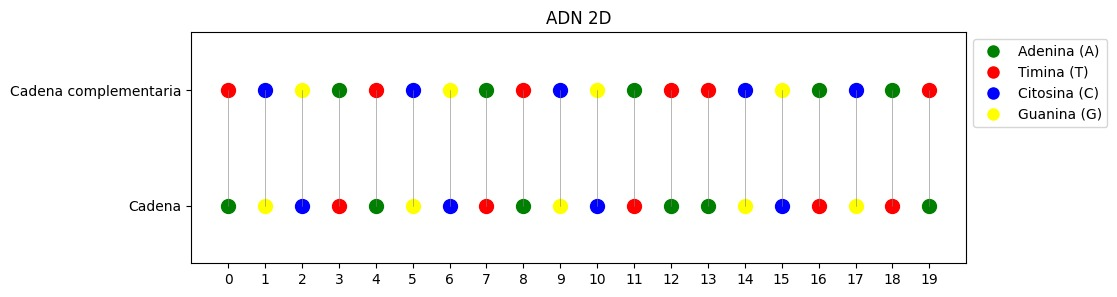
\includegraphics[scale=0.25]{adn1.jpeg} 
    \end{figure}

Aunque no utilizaremos este proceso en los siguientes pasos, mostramos cómo se realiza la transcripción de ADN a ARN y cómo se traduce el ARN a proteínas.

\begin{lstlisting}[language=Python]
arn = cadena_adn.transcribe()
print(f"Secuencia ARN: {arn}")

proteina = arn.translate()
print(f"Proteina: {proteina}")
\end{lstlisting}
Ilustrando un poco como se realiza la transcripción de ADN a ARN hicimos el siguiente gráfico
\begin{figure}[h]
\centering
        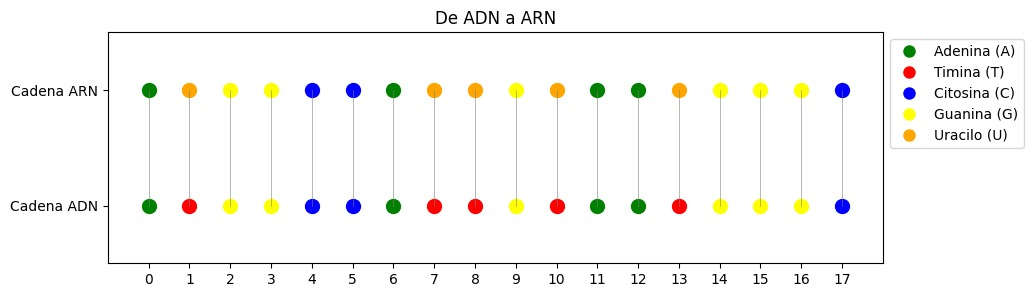
\includegraphics[scale=0.25]{arn.png} 
    \end{figure}
Utilizando todas las librerias anteriormente mencionadas realizamos la representación gráfica de la proteina a la que se puede transcribir la cadena de ARN (estas imágenes puede verlas en el archivo de código).\\


\subsection{Codificación y Decodificación con Códigos Reed-Solomon y Hamming}

En esta sección, nos adentramos en la parte central de nuestro trabajo, donde realizamos una codificación y decodificación utilizando los códigos Reed-Solomon y Hamming.

\subsubsection{Ejemplo de Corrección de Errores con Reed-Solomon}
Para ilustrar este proceso, comenzamos con un ejemplo de transcripción de ADN a ARN, donde introducimos errores en la secuencia de ARN. Luego, utilizamos los códigos Reed-Solomon para corregir estos errores, simulando el mecanismo de corrección que ocurre en la naturaleza.

\begin{lstlisting}[language=Python]
import unireedsolomon as rs
from random import choice, randint

def generar_adn(longitud):
    nucleotidos = "ATCG"
    return ''.join(choice(nucleotidos) for _ in range(longitud))

def adn_a_arn(adn):
    return adn.replace('T', 'U')


def introducir_mutaciones(sec, num_mutaciones):
    sec_lista = list(sec)
    nucleotidos = "AUCG"
    for _ in range(num_mutaciones):
        pos = randint(0, len(sec_lista) - 1)
        nucleotido_original = sec_lista[pos]
        nucleotidos_posibles = nucleotidos.replace(nucleotido_original, '')
        sec_lista[pos] = choice(nucleotidos_posibles)
    return ''.join(sec_lista)


n = 19  
k = 15  

coder = rs.RSCoder(n, k)


adn_original = generar_adn(15)
print(f"ADN original: {adn_original}")


arn_original = adn_a_arn(adn_original)
print(f"ARN original: {arn_original}")

arn_codificado = coder.encode(arn_original)
print(f"ARN codificado (hex): {arn_codificado.encode('latin1').hex()}")


arn_con_mutaciones = introducir_mutaciones(arn_codificado, 2)  # Introducir 2 mutaciones
print(f"ARN con mutaciones: {arn_con_mutaciones}")


try:
    arn_corregido, errores_corregidos = coder.decode(arn_con_mutaciones)
    print(f"ARN corregido: {arn_corregido}")
    print(f"Errores corregidos: {errores_corregidos}")
except rs.RSCodecError as e:
    print(f"Error: No se pudieron corregir todos los errores. {e}")
\end{lstlisting}

En este código se genera una cadena de ADN aleatoria de longitud especificada y esta se transcribe a ARN, reemplazando las timinas (T) por uracilos (U). Posteriormente, se introducen mutaciones en la secuencia de ARN para simular errores en la transcripción, la secuencia de ARN se codifica utilizando el código Reed-Solomon, que añaden $4$ bits de paridad para la detección y corrección de errores.\\

Este proceso es análogo a lo que ocurre en la naturaleza durante la transcripción del ADN. La enzima polimerasa revisa y corrige los errores que puedan ocurrir durante la replicación del ADN, asegurando que la información genética se transmita de manera precisa. En nuestro caso, los códigos Reed-Solomon actúan como la polimerasa, corrigiendo los errores introducidos en la secuencia de ARN.\\


En este ejemplo, el número de mutaciones introducidas es estático (2 mutaciones), ya que la idea es acercarse lo más posible a la realidad biológica. En la naturaleza, la probabilidad de que ocurran errores durante la transcripción es baja, y los mecanismos de corrección son altamente eficientes. Por esta razón, no se utilizó una matriz de transición para introducir mutaciones de manera probabilística, ya que esto reduciría la probabilidad de decodificación correcta, algo que no ocurre en el ADN.




\subsubsection{Aplicación Práctica: Codificación y Decodificación de una Palabra}

Para mostrar una aplicación análoga a lo que hace el ADN en la realidad, codificamos una palabra utilizando el código Reed-Solomon. Es importante destacar que las codificaciones no se aplican a los bits de paridad, y para utilizar completamente la librería \texttt{unireedsolomon}, realizamos una serie de conversiones. Primero, convertimos la cadena de texto a ASCII, luego a base 4, asignamos nucleótidos de ADN, introducimos ruido mediante una matriz de transición, y finalmente realizamos las conversiones inversas para decodificar la palabra. La idea principal del código es,

\begin{lstlisting}[language=Python]
palabra = input("Ingrese una palabra: ")


ascii_palabra = palabra_a_ascii(palabra)
print(f"Palabra en ASCII: {ascii_palabra}")


polinomio_palabra = polinomio(ascii_palabra)
print(f"Palabra en polinomio: {polinomio_palabra}")


def arreglar_palabra(palabra):
    palabra_coder = ''
    for i in ascii_palabra:
        palabra_coder = palabra_coder + i
    num_coder = int(palabra_coder[0:len(palabra_coder)])
    return palabra_coder

palabra_coder = arreglar_palabra(ascii_palabra)


n = len(palabra_coder) + 4
k = len(palabra_coder)


coder = rs.RSCoder(n, k)


ascii_codificado = coder.encode(palabra_coder)
print(f"Palabra codificada: {ascii_codificado}")


base4_codificado = ascii_a_base4(ascii_palabra)
print(f"Palabra codificada en base 4: {base4_codificado}")


adn_codificado = base4_a_adn(base4_codificado)
print(f"Palabra codificada en ADN: {adn_codificado}")


matriz_transicion = [
    [0.98, 0.005, 0.005, 0.01], 
    [0.005, 0.005, 0.98, 0.01], 
    [0.01, 0.005, 0.005, 0.98]   
]


adn_con_errores = introducir_errores_con_matriz(adn_codificado, matriz_transicion)
print(f"ADN con errores: {adn_con_errores}")

base4_con_errores = nucleotidos_a_base4(adn_con_errores)
print(f"Base 4 con errores: {base4_con_errores}")

ascii_con_errores = base4_a_ascii(base4_con_errores)
print(f"ASCII con errores: {ascii_con_errores}")

ascii_con_errores = ascii_con_errores + ascii_codificado[len(ascii_codificado) - 4:len(ascii_codificado)]
print(f"ASCII con errores y paridad: {ascii_con_errores}")

try:
    palabra_corregida = coder.decode(ascii_con_errores)
    print(f"Palabra corregida: {palabra_corregida}")
    palabra_final = ascii_a_palabra(palabra_corregida[0], ascii_palabra)
    print(f"Palabra final: {palabra_final}")
\end{lstlisting}

La palabra ingresada se convierte a su representación en ASCII, lo que permite trabajar con valores numéricos, los valores ASCII se convierten a base 4, lo que facilita la asignación de nucleótidos de ADN.Cada dígito en base 4 se asigna a un nucleótido (A, T, C, G) posteriormente, se utiliza una matriz de transición para introducir errores en la secuencia de ADN, simulando mutaciones.Por último se realizan las conversiones inversas para obtener la palabra original, corrigiendo los errores introducidos mediante el código Reed-Solomon.



